\documentclass[aspectratio=169]{beamer}
\usepackage{fontawesome}
\usepackage{hyperref}
\usepackage{url}
\usepackage{tikz}
\usetheme{Madrid}
\usecolortheme{sidebartab}
\usefonttheme{professionalfonts}
\urlstyle{same}


\title{Ansible for Network Automation}
\subtitle{Ansible Configuration and Verification}
\date{}
\author{Josh VanDeraa}

\begin{document}
\begin{frame}
  \maketitle
  \footnotesize
  \faTwitter vanderaaj \hfill \faGithub jvanderaa \hfill \faSlack jvanderaa
\end{frame}

\begin{frame}
    \frametitle{Session Overview}
    At the end of this session you will have seen how to:
    \begin{itemize}
      \item <2-> Setup of a new role
      \item <3-> Use a role in a playbook
    \end{itemize}
  \end{frame}

  \begin{frame}[t]
    \frametitle{Roles - What are they}
      \begin{itemize}
        \item <2-> Roles load items only during the load of the role
        \item <3-> More separation of tasks
        \item <4-> Easier to share the roles, with help from Ansible Galaxy
        \begin{itemize}
          \item <4-> Ansible Galaxy is the repository of roles and collections
          \item <5-> Roles that get published to be shared - recall the earlier session
          \item <6-> Collections are new in 2.9 and include playbooks, roles, modules, and plugins in one
        \end{itemize}
      \end{itemize}
  \end{frame}

  \begin{frame}
    \frametitle{Network Diagram}
    \begin{center}
        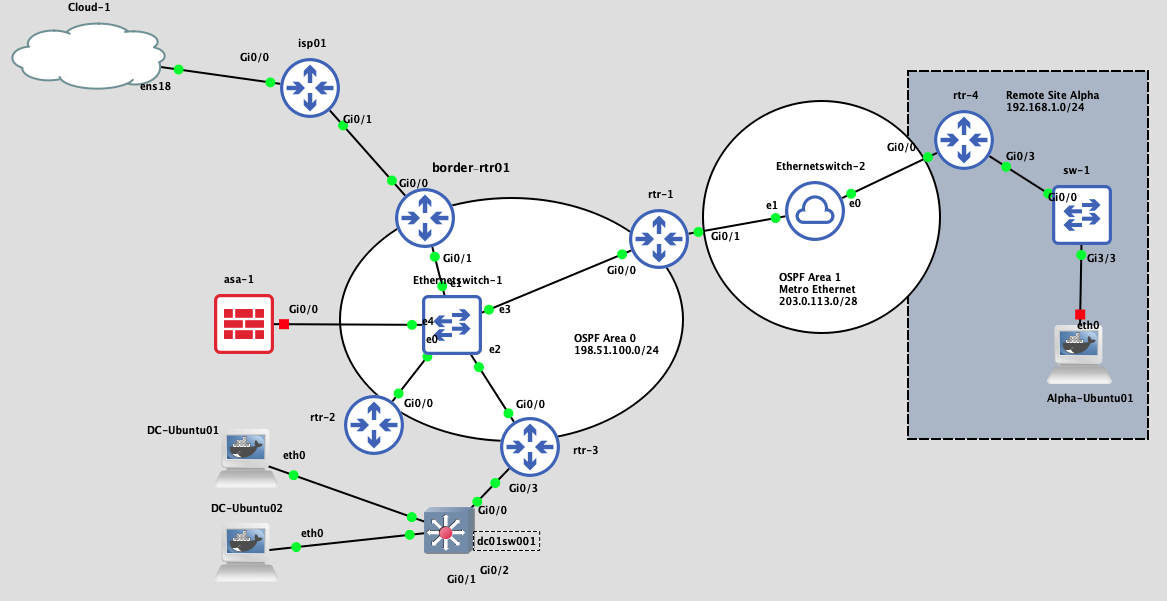
\includegraphics[height=0.8\paperheight]{assets/web_server_setup.png}    
    \end{center}
  \end{frame}

  \begin{frame}
    \frametitle{DEMO!}
    \begin{columns}
    \begin{column}{0.3\textwidth}
      \Huge
      \begin{center}
        \faDesktop 
        \hspace{.5cm}
        \faRocket     
      \end{center}
    \end{column}
    \begin{column}{0.7\textwidth}
      \huge 
        Let's take a look!
        \begin{itemize}
          \item Full configuration and verification of QoS
        \end{itemize}
    \end{column}
    \end{columns}
  \end{frame}

  \begin{frame}
    \frametitle{Summary}
      To review what we accomplished today:
      \begin{itemize}
        \item <2-> Demonstrated how to build the folder structure of a role with ansible-galaxy
        \item <3-> Changed QoS of traffic in the lab network
        \item <4-> Verification of changes using show commands with a delay
      \end{itemize}
  \end{frame}

  \begin{frame}
    \frametitle{Contact}
    \huge
    \begin{center}
      \url{https://packetpushers.slack.com}
    \end{center}
    \begin{center}
      \normalsize
      \faSlack \hspace{.1cm}jvanderaa  
    \end{center}
  \end{frame}

\end{document}